% !TEX root =../LibroTipoETSI.tex
\chapter{Protocolo MQTT y STOMP}\LABCHAP{MQTT}
\pagestyle{esitscCD}

\section{MQTT}

\texttt{MQTT} es un protocolo cliente/servidor que permite roles de publicador/suscriptor.
Es ligero, abierto, simple y diseñado para ser fácil de implementar en el cliente.
Estas características lo hacen ideal para su uso en múltiples situaciones, como por ejemplo,
entornos donde la memoria y el ancho de banda son limitados, como la comunicación M2M
(\emph{Machine to machine}) o para dispositivos en el Internet de las Cosas.

Es un protocolo binario ligero que, en comparación con \texttt{HTTP}, tiene una
mínima sobrecarga en cuanto a cabeceras para hacer más eficiente el tampaño de los
paquetes.
\texttt{MQTT} es muy fácil de implementar en el cliente. Esto encaja perfectamente
en sistemas integrados con recursos limitados, de hecho,
esto es uno de los objetivos que se buscaban cuando \texttt{MQTT} se creó.

\subsection{El patrón publicador/suscriptor}

\begin{figure}[htbp]
\centering
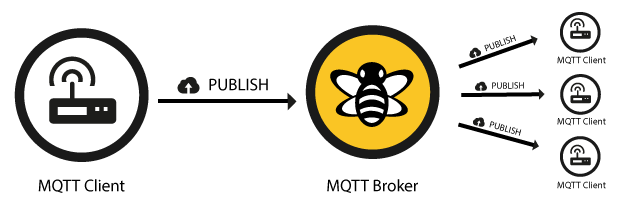
\includegraphics[width=\linewidth]{03-mqtt_stomp_amqp/figuras/fig001}
\caption{Patrón publicador/suscriptor}
\label{fig:figura1}
\end{figure}

El patrón publicador/suscriptor es una alternativa al sistema tradicional de
cliente/servidor, donde un cliente se comunica directamente con un destino.
Sin embargo, el patrón \texttt{pub/sub} desacopla al cliente que están enviando
un mensaje (publicador) de otro cliente o más clientes que reciben mensajes
(suscriptor). Esto quiere decir que publicador y suscriptor no son conscientes
de la existencia del otro. Existe un tercer componente llamado \emph{broker} que
es conocido tanto por el publicador como el suscriptor que es el encargado de
filtrar los mensajes que llegan y distribuirlos correctamente.

As already mentioned the main aspect in pub/sub is the decoupling of publisher and receiver, which can be differentiated in more dimensions:
Como ya hemos mencionado, el pricipal aspecto del patrón publicador/suscriptor
es el desacople en las siguientes dimensiones:

\begin{itemize}\itemsep1pt \parskip0pt \parsep0pt
\item Espacio desacoplado: Publicador y suscriptor no tiene porqué saber el uno del otro (IP, puerto, etc.).
\item Tiempo desacoplado: Publicador y suscriptor no tienen porqué estar en ejecución al mismo tiempo.
\item Sincronización desacoplada: Las operaciones de los dos componentes no se detienen durante envío o recepción.
\end{itemize}

En resumen, el patrón publicador/suscriptor desacopla el publicador o receptor de
un mensaje y a través de los filtros para los mensajes se puede elegir qué clientes
reciben qué mensajes.

\subsection{Escalabilidad}

El patrón publicador/suscriptor ofrece mejor escalabilidad que el patrón clásico
de cliente/servidor. Esto se debe a que las operaciones en el broker pueden ser
altamente paralelizadas. También es común el cacheo de mensajes y el enrutado
inteligente. Sin embargo, es un reto el escalar a millones de conexiones, esto
puede conseguirse mediante el uso de clústeres de \emph{brokers} para distribuir
la carga entre múltiples servidores.

\subsection{Filtrado de mensajes}

El filtrado de mensajes es el encargado de que sólamente los mensajes sean
recibidos por los clientes que deben. Tenemos varias opciones de filtrado de
mensajes:

\begin{itemize}\itemsep1pt \parskip0pt \parsep0pt
\item Filtrado basado en \texttt{topic}: El \texttt{topic} puede ser parte de cada mensaje. Cada
cliente recibe sólamente mensajes del \texttt{topic} en el que está interesado. Los topics
generalmente son cadenas de texto organizadas de forma jerárquica, por lo que se puede
filtrar en función de una expresión.
\item Filtrado basado en contenido: El filtrado se basa en el contenido específico
del mensaje. Una gran desventaja de este método es que el contenido del mensaje
debe ser conocido por el \emph{broker}, cosa que no siempre ocurre, por ejemplo,
cuando el contenido va cifrado.
\item Filtrado por tipo: En lenguajes orientados a objetos es típico filtrar en
base a un tipo o clase del mensaje o evento. En este caso el suscriptor podría
recibir todos los mensajes de un tipo o subtipo.
\end{itemize}

En el caso de \texttt{MQTT} se utiliza el filtrado por \texttt{topic} así que cada
mensaje contiene un \texttt{topic}, el cual es procesado por el \texttt{broker}
para entregarlo a los clientes que se han suscrito a él.

\texttt{MQTT} tiene múltiples niveles de calidad de servicio (QoS). Se puede
conseguir fácilmente que un mensaje sea entregado del cliente al \emph{broker} o
del \emph{broker} al cliente. Sin embargo, existe la posibilidad de que nadie
se suscriba a un \texttt{topic} en particular, en este caso depende el \emph{broker}
cómo se debe manejar la situación.

\subsection{Diferencias con un sitema de colas}

Existe confusión debido a su nombre en cuanto a sí es un protocolo de colas.
Su nombre proviene de \emph{MQseries}, un producto de \emph{IBM} y no de \emph{Message Queue}.
Independientemente del nombre, existen diferencias entre \texttt{MQTT} y un
sistema de colas:

\begin{itemize}\itemsep1pt \parskip0pt \parsep0pt
\item Un sistema de colas almacena un mensaje hasta que se consume: En un sistema
clásico los mensajes se almacenan hasta que son tomados por un cliente (consumidor),
esto en \texttt{MQTT} no ocurre ya que puede haber cero clientes suscritos a un
topic y el mensaje es descartado.
\item Un mensaje sólo es consumido por un cliente: Otra gran diferencia es el hecho
de que en un sistema tradicional de cola de mensajes, los mensajes son consumidos
por un único consumidor así la carga se puede distribuir entre múltiples procesos.
En \texttt{MQTT} esto suele ser al contrario, todos los suscriptores reciben el
mensaje si se han suscrito al \texttt{topic}.
\item Las colas tienen nombres y deben crearse de forma explícita: Una cola es
menos flexible que un \emph{topic}, antes de usar una cola debe declarase
explícitamente y sólo entonces se pueden consumir los mensajes. En \texttt{MQTT}
los \emph{topics} son extremadamente flexibles y son creados en el momento.
\end{itemize}

\section{STOMP}

\texttt{STOMP} (\emph{Simple Text Orientated Messaging Protocol}), a diferencia
de \texttt{MQTT}, está orientado a texto, como \texttt{HTTP}. El protocolo permite
a clientes conectarse a un \emph{broker} para que se puedan comunicar fácilmente
entre diferentes tipos de aplicaciones y plataformas.
En \texttt{STOMP} también se sigue un modelo publicador/suscriptor.

Se centra en tener un diseño simple y minimalista y que sea muy fácil de
implementar en cualquier lenguaje. Al funcionar en modo texto, hacer un cliente
puede ser tan sencillo como abrir una sesión \texttt{Telnet} para loguearse
en cualquier \emph{broker} de \texttt{STOMP} e interaccionar con él. Se dice
que es posible crear un cliente de \texttt{STOMP} en un par de horas.

\section{AMQP}

AMQP (Advanced Message Queuing Protocol) es un protocolo de mensages que permite
a aplicaciones de clientes comunicarse con un broker.

\subsection{Brokers}

Los brokers de mensajes reciben los mensajes de los publicadores (aplicaciones
que los publican, también conocidos como productores) y los enrutan hacia los
consumidores (aplicaciones que los procesan).

Ya que es un protocolo de red, los publicadores, consumidores y el broker pueden
residir en diferentes máquinas.

\subsection{El modelo AQMP}

El modelo de AMQP 0-9-1 tiene la siguiente visón de lo que ocurre:

Los mensajes se publican en \emph{exchanges}, que se podrían ver como un buzón
o una oficina postal. Los \emph{exchanges}, al recibir mensajes, los distribuyen
a las colas (\emph{queues}) siguiendo unas reglas llamadas \texttt{bindings}.
A continuación, el \emph{broker} entrega los mensajes a los consumidores
que están suscritos a las colas, o los propios consumidores consultan la cola
y leen los mensajes.

\begin{figure}[htbp]
\centering
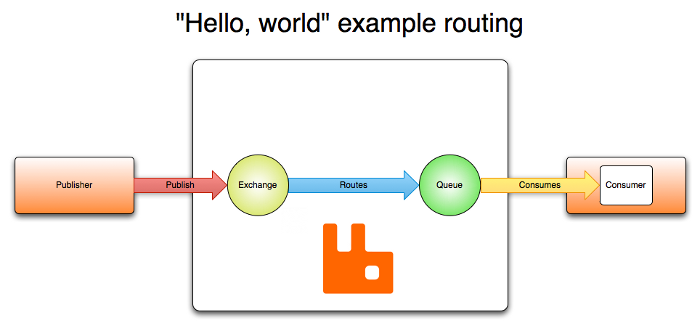
\includegraphics[width=\linewidth]{03-mqtt_stomp_amqp/figuras/fig002}
\caption{Ejemplo de enrutamiento en AMQP}
\label{fig:figura2}
\end{figure}

Cuando se publica un mensaje, se pueden especificar diferentes atributos (\emph{metadata}).
Alguno de estos atributos pueden ser usados por el \emph{broker}, sin embargo,
el cuerpo del mensajes es completamente opaco para el \emph{broker} y sólamente
será usado por la aplicación que recibirá el mensaje.

Las redes pueden tener problemas y las aplicaciones puede fallas al procesar los
mensajes, por eso mismo, el modelo \texttt{AMQP} hace uso de \texttt{ACKs}. Cuando
un mensaje se entrega a un consumidor, éste debe notificar al broker que ha procesado
el mensaje, ya sea de forma automática o cuando el desarrollador de la aplicación
lo decida. El \emph{broker} sólamente eliminará el mensaje de la cola cuando
éste haya sido confirmado.

En algunas situaciones, por ejemplo, cuando un mensaje no puede ser enrutado,
el mensaje puede ser devuelto al productor, descartado o, si el broker lo implementa,
enviado a una cola especial llamada \emph{dead letter queue}. Los consumidores pueden
elegir cómo manejar situaciones como estas usando algunos parámetros a la hora de
publicar los mensajes.

Las colas, los \emph{exchanges} y los \emph{bindings} son conocidas como
\textbf{entidades de AMQP}-

\subsection{\emph{Exchanges}}

Los \emph{exchanges} son entidades de AMQP a donde llegan los mensajes. Éstos
al recibir los mensajes los enrutan hacia cero o más colas. El algoritmo de
enrutado depende del tipo de \emph{exchange} y las reglas definidas (\emph{bindings}).
Existen cuatro tipos de \emph{exchanges}:

\begin{itemize}\itemsep1pt \parskip0pt \parsep0pt
\item Direct exchange: \texttt{amq.direct}
\item Fanout exchange: \texttt{amq.fanout}
\item Topic exchange:	\texttt{amq.topic}
\item Headers exchange:	\texttt{amq.match}
\end{itemize}

Independientemente del tipo de \emph{exchange}, éstos son declarados con ciertos
atributos, los más importantes son:

\begin{itemize}\itemsep1pt \parskip0pt \parsep0pt
\item Name: Nombre del \emph{exchange}.
\item Durability: Indica al \emph{broker} que debe sobrevivir a
reinicios.
\item Auto-delete: Son eliminados sin no hay ninguna cola asociada.
\item Arguments: Dependen del \emph{broker}.
\end{itemize}

\subsubsection{\emph{Direct Exchange}}

Los \emph{exchanges} directos entregan los mensajes a las colas basándose en
la \texttt{routing key}. Son ideales para enrutamiento \emph{unicast}, aunque
también se pueden usar para \emph{multicast}. Funcionan de la siguiente manera:

\begin{itemize}\itemsep1pt \parskip0pt \parsep0pt
\item Una cola se conecta (establece un \emph{binding}) al \emph{exchange} con
la \texttt{routing key} \texttt{K = R}
\item El \emph{exchange} directo suele ser usado para distribuir mensajes entre
múltiples \emph{workers} en modo \emph{round robin}. Es importante ser conciente
de que en \texttt{AMQP} se balancea entre consumidores y no entre colas.
\end{itemize}

Se puede ver de forma grágica en la \FIG{figura2}.

\begin{figure}[htbp]
\centering
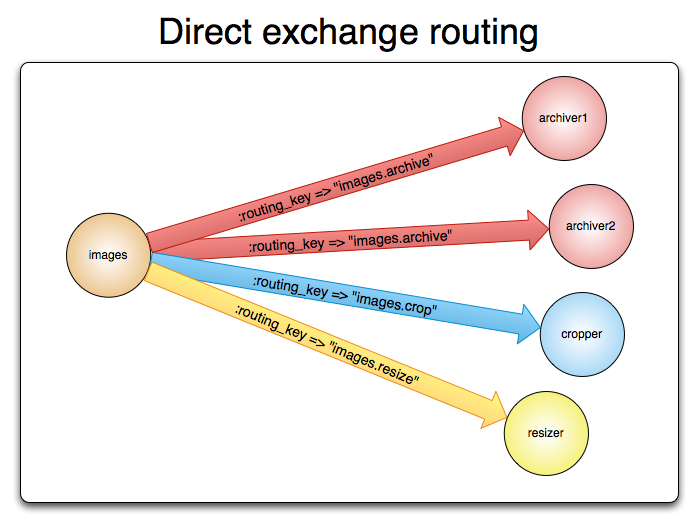
\includegraphics[width=0.75\linewidth]{03-mqtt_stomp_amqp/figuras/fig003}
\caption{\emph{Exchange} directo}
\label{fig:figura3}
\end{figure}

\subsubsection{\emph{Fanout Exchange}}

Este tipo de \emph{exchange} enruta todos los mensajes a todas las colas con las
que está conectado, es decir, la \texttt{routing key} se ignora en este caso.
Una copia de cada mensaje es enviado a cada una de las colas. Este tipo de
\emph{exchange} es ideal para el tráfico \emph{broadcast}.

Se puede ver de forma grágica en la \FIG{figura4}.

\begin{figure}[htbp]
\centering
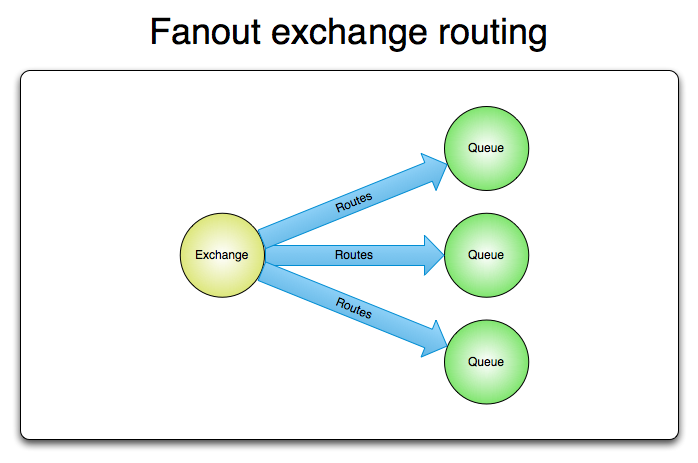
\includegraphics[width=0.75\linewidth]{03-mqtt_stomp_amqp/figuras/fig004}
\caption{\emph{Fanout exchange}}
\label{fig:figura4}
\end{figure}

\subsubsection{\emph{Topic Exchange}}

En este caso, los mensajes se envían a una o varias colas, basándose en la
\texttt{routing key} con la que una cola está conectada a un \emph{exchange}. Este
patrón se suele usar en modelos de publicador/suscriptor.

\subsubsection{\emph{Header Exchange}}

El \emph{header echange} está diseñado para enrutar mensajes basándose en múltiples
atributos que viajan en las cabeceras de los mensajes en lugar de usar la
\texttt{routing key}.

\subsection{Colas}

Las colas en \texttt{AMQP} son muy similares a las colas en otros sistemas de
colas. Almacenan mensajes que pueden se consumidos por aplicaciones. Las colas
comparten algunas propiedades con los \emph{exchanges}, pero también tienen sus
propios atributos:

\begin{itemize}\itemsep1pt \parskip0pt \parsep0pt
\item Name: Nombre de la cola.
\item Durable: Indica al \emph{broker} que deben sobrevivir a
reinicios.
\item Exclusive: Sólo se permite una conexión a la cola.
\item Arguments: Dependen del \emph{broker}.
\end{itemize}

Las colas deben ser declaradas antes de poder ser usadas. La declaración hace que
la cola se cree si no existía anteriormente, si ya estuviese declarada, otra
declaración no tendrá ningún efecto. Si se vuelve a declarar con otros atributos
diferentes, se producirá una excepción.

\subsubsection{Colas durables}

Las colas durables se persisten a disco y sobreviven a reinicios del \emph{broker},
en cambio, las colas que no son durables son llamadas transitorias. No todos los
escenarios requieren que una cola sea durable.

La durabilidad de una cola no hace que los mensajes que sean enrutados hacia esa
cola sean durables. Si el \emph{broker} se reinicia, las colas durables volverán
a declararse durante el inicio de forma automática, sin embargo, sólamente los
mensajes persistidos podrán recuperarse.

\subsection{\emph{Bindings}}

Los \emph{bindings} son reglas usadas por los \emph{exchanges} para enrutar los
mensajes recibidos hacia las colas. Para que un \emph{exchange} enrute un mensaje
a una cola, dicha cola debe enlazarse con el \emph{exchange}. Los \emph{bindings}
pueden tener atributos opcionales como las \texttt{routing keys}. La finalidad
de una clave de enrutado es seleccionar ciertos mensajes publicados en un \emph{exchage}
que está enlazado con una cola, es decir, actúan como filtros.

Cuando un mensaje no se puede enrutar hacia una cola se descartará o se devolverá
al productor, dependiendo de los atributos que el productor haya ajustado.

\subsection{Mensages}

Los mensajes en \texttt{AMQP} tienen atributos. Algunos de ellos son tan común
que la especificación los define de forma que los desarrolladores no tienen que
preocuparse por ellos.

\begin{itemize}\itemsep1pt \parskip0pt \parsep0pt
\item Content type
\item Content encoding
\item Routing key
\item Delivery mode
\item Message priority
\item Message publishing timestamp
\item Expiration period
\item Publisher application id
\end{itemize}

Algunos atributos los usa el \emph{broker}, pero la mayoría de ellos son para
los consumidores que lo reciben. Algunos atributos
son opcionales. Los atributos se fijan cuando el mensaje se publica.

Los mensajes también tienen una carga (los datos) que el \emph{broker} trata
como una ristra de \emph{bytes}. El \emph{broker} no inspecciona o modifica
los datos. Es bastante común enviar los datos serializados en formatos como
\texttt{JSON}, \texttt{MessagePack}, \texttt{Protocol BUffers}, etc. Para comunicar
esta información se pueden usar los atributos \texttt{content-type} o \texttt{content-encoding}.

Los mensajes pueden ser publicados como persistentes, que hace que el \emph{broker}
los persista a disco. Si el servidor se reinicia, el sistema se asegura que los
mensajes persistentes no se pierdan. Sólo por publicar un mensaje en un \emph{exchange}
durable o que la cola a la que el mensaje es enrutado sea durable no hace que el
mensaje sea persitido, para ello el mensaje tiene que ser publicado como persistente.
Hay que tener en cuenta que publicar mensajes persistentes afecta al rendimiento.


\section{STOMP vs. MQTT vs. AMQP}

Como se puede ver, \texttt{STOMP} y \texttt{MQTT} son protocolos muy semejantes,
entonces, ¿Cuándo usaremos cada uno de ellos?. Pues los dispositivos usarán el
protocolo \texttt{MQTT} ya que ofrece más funcionalidad y es muy fácil encontrar
implementaciones para muchos tipos de dispositivos.

Sin embargo, para el lado de las aplicaciones se ha decidido usar \texttt{STOMP}.
Esto quiere decir, que las aplicaciones del usuario que deseen conectarse al
sistema para obtener los datos que los dispositivos envían mediante \texttt{MQTT}
deben hacerlo usando \texttt{STOMP}. Esto es así porque una de las cosas que
permite \texttt{STOMP} es que puede usar cualquier capa de transporte. Uno de los
requisitos que se busca es que un navegador web pueda conectarse
directamente a la plataforma y recibir datos. De esta forma no se requeriría que
el servidor de la aplicación web obtenga los datos y los envíe al navegador, es decir,
se pueden hacer aplicaciones \emph{serverless}.

Desde un navegador web sólo se permite el tráfico \texttt{HTTP}, por lo que, en
principio, no se puede usar \texttt{MQTT} ya que este viaja en \texttt{TCP}. Ahí
es donde entra en juego \texttt{STOMP}, que está diseñado para funcionar independientemente
de la capa que haya debajo, lo que lo hace ideal para funcionar sobre \texttt{websockets}.

Dicho esto el escenario es el siguiente:

\begin{itemize}\itemsep1pt \parskip0pt \parsep0pt
\item Los dispositivos se conectan mediante \texttt{MQTT} sobre \texttt{TCP} a
la plataforma. Se suscriben y publican en \emph{topics}.
\item Las aplicaciones de la lógica del usuario se conecta a la plataforma usando
\texttt{STOMP} bien sobre una sesión \texttt{TCP} o bien sobre \emph{websockets}
en caso de que quien realice la conexión sea un navegador. Se suscriben y publican
en \emph{topics}.
\item La plataforma, de forma interna, convierte los mensajes \texttt{MQTT} y
\texttt{STOMP} a \texttt{AMQP} y trabaja con este sistema de forma interna.
Veremos qué es \texttt{AMQP} en el siguiente capítulo.
\end{itemize}
